% Pandoc LaTeX template — ACME arXiv paper
% Page 1: single-column title + abstract; body: two columns
\documentclass[11pt,a4paper]{article}

\usepackage{fontspec}
\IfFontExistsTF{Libertinus Serif}{%
  \setmainfont{Libertinus Serif}%
}{%
  \IfFontExistsTF{Times New Roman}{%
    \setmainfont{Times New Roman}%
  }{%
    \setmainfont{Latin Modern Roman}%
  }%
}
\IfFontExistsTF{Libertinus Sans}{%
  \setsansfont{Libertinus Sans}%
}{%
  \IfFontExistsTF{Helvetica Neue}{%
    \setsansfont{Helvetica Neue}%
  }{%
    \setsansfont{Latin Modern Sans}%
  }%
}
\setmonofont{Menlo}[Scale=0.85]

\usepackage{geometry}
\geometry{
  top=0.95in,
  bottom=0.95in,
  left=0.85in,
  right=0.85in,
  columnsep=0.28in
}

\usepackage[dvipsnames]{xcolor}
\usepackage{hyperref}
\hypersetup{
  colorlinks=true,
  linkcolor=NavyBlue,
  urlcolor=NavyBlue,
  citecolor=NavyBlue,
  pdfauthor={Mohamed Kamil Bourouiba},
  pdftitle={ACME: Adaptive Cognitive Memory Engine}
}

\usepackage{setspace}
\setstretch{1.08}
\usepackage{parskip}
\setlength{\parskip}{0.42em plus 0.1em minus 0.08em}

\usepackage{titlesec}
\titleformat{\section}
  {\sffamily\large\bfseries}{\thesection.}{0.6em}{}
\titleformat{\subsection}
  {\sffamily\normalsize\bfseries}{\thesubsection}{0.6em}{}
\titleformat{\subsubsection}
  {\sffamily\normalsize\bfseries\itshape}{}{0em}{}
\titlespacing*{\section}{0pt}{2.4ex plus 1ex minus .2ex}{1.1ex plus .2ex}
\titlespacing*{\subsection}{0pt}{1.8ex plus .8ex minus .2ex}{0.8ex plus .2ex}
\titlespacing*{\subsubsection}{0pt}{1.4ex plus .6ex minus .2ex}{0.5ex plus .2ex}

\usepackage{booktabs}
\usepackage{array}
\usepackage{multirow}
\usepackage{calc}
\usepackage{colortbl}
\usepackage{siunitx}
\usepackage{makecell}
\usepackage{adjustbox}
\usepackage{needspace}
\usepackage{placeins}
\usepackage{tikz}
\usetikzlibrary{arrows.meta, positioning, shapes.geometric, fit, backgrounds, calc}
\usepackage{tcolorbox}
\tcbuselibrary{skins,breakable}

\renewcommand{\arraystretch}{1.35}
\setlength{\tabcolsep}{7pt}

\usepackage{microtype}
\usepackage{enumitem}
\setlist[itemize]{topsep=0.35em, itemsep=0.2em, parsep=0pt, leftmargin=1.4em}
\setlist[enumerate]{topsep=0.35em, itemsep=0.2em, parsep=0pt, leftmargin=1.4em}

\renewenvironment{abstract}{%
  \vspace{0.2em}%
  \begin{center}%
  \begin{minipage}{0.92\linewidth}%
  \textbf{\large\sffamily Abstract}\par\vspace{0.55em}%
  \itshape\small%
}{%
  \end{minipage}%
  \end{center}%
  \vspace{0.85em}%
}

\definecolor{keybg}{RGB}{245,248,252}
\definecolor{keyborder}{RGB}{0,82,120}
\definecolor{acmefigblue}{RGB}{0,82,120}
\definecolor{acmefiggray}{RGB}{100,110,125}
\definecolor{acmefiglight}{RGB}{235,242,248}
\definecolor{acmein}{RGB}{228,240,250}
\definecolor{acmemem}{RGB}{220,236,228}
\definecolor{acmereason}{RGB}{248,240,225}
\definecolor{acmefb}{RGB}{238,228,246}
\definecolor{acmerow}{RGB}{232,240,248}
\definecolor{bannerbg}{RGB}{241,245,249}

\newtcolorbox{keyfinding}{%
  enhanced,
  breakable,
  colback=keybg,
  colframe=white,
  boxrule=0pt,
  borderline west={2.5pt}{0pt}{keyborder},
  left=7pt, right=7pt, top=5pt, bottom=5pt,
  before skip=0.85em,
  after skip=0.95em,
  fontupper=\small
}
\newtcolorbox{contributions}{%
  enhanced,
  colback=keybg,
  colframe=keyborder!50,
  boxrule=0.35pt,
  arc=2pt,
  left=8pt, right=8pt, top=6pt, bottom=6pt,
  fonttitle=\sffamily\bfseries\small,
  title={Contributions},
  before skip=0.6em,
  after skip=0.85em,
  fontupper=\small
}
\newtcolorbox{metabox}{%
  enhanced,
  colback=bannerbg,
  colframe=keyborder!25,
  boxrule=0.3pt,
  arc=3pt,
  left=10pt, right=10pt, top=6pt, bottom=6pt,
  before skip=0pt,
  after skip=0pt
}
\newtcolorbox{bannerbox}{%
  enhanced,
  colback=bannerbg,
  colframe=keyborder!35,
  boxrule=0.35pt,
  arc=4pt,
  left=8pt, right=8pt, top=7pt, bottom=7pt,
  halign=center
}

\newcommand{\acmeTitleStrip}{%
  \begin{bannerbox}
    \small\sffamily\color{keyborder}
    LLM \textrightarrow\ Episodic Memory \textrightarrow\ Belief Engine \textrightarrow\
    Feedback Loop \textrightarrow\ Updated Beliefs
  \end{bannerbox}%
}

\providecommand{\tightlist}{%
  \setlength{\itemsep}{0pt}\setlength{\parskip}{0pt}}

\usepackage{caption}
\captionsetup{skip=0.55em, labelfont={bf,sf}, font=small}
\captionsetup[table]{position=above,skip=0.3em}

\usepackage{fvextra}
\DefineVerbatimEnvironment{Highlighting}{Verbatim}{breaklines,commandchars=\\\{\},xleftmargin=0.5em,fontsize=\footnotesize}

\clubpenalty=3000
\widowpenalty=3000
\displaywidowpenalty=3000

\newcommand{\acmeBackMatterBegin}{%
  \FloatBarrier
  \clearpage
  \onecolumn
}
\newcommand{\acmeReferencesBegin}{%
  \small
  \setlength{\parskip}{0.32em}%
  \setlength{\parindent}{-1.15em}%
  \setlength{\leftskip}{1.15em}%
}
\newcommand{\acmeReferencesEnd}{%
  \normalsize
  \setlength{\parindent}{0pt}%
  \setlength{\leftskip}{0pt}%
}

\sisetup{
  table-format=1.3,
  table-number-alignment=right,
  detect-weight=true,
  detect-family=true
}

\newcommand{\acmeTableHdr}{%
  \textbf{System} &
  {\textbf{Ret.}} &
  {\textbf{Gnd.}} &
  {\textbf{Fbk.}} &
  {\textbf{Bel.}} &
  {\textbf{Ovr.}} \\%
}

% Multi-line benchmark column headers (positioning tables)
\newcommand{\acmeBenchCols}{%
  \textbf{Capability} &
  \makecell[c]{\textbf{LongMem}\\\textbf{Eval}} &
  \makecell[c]{\textbf{MemAgent}\\\textbf{Bench}} &
  \makecell[c]{\textbf{Reflection}\\\textbf{Bench}} &
  \makecell[c]{\textbf{Mem}\\\textbf{Bench}} &
  \makecell[c]{\textbf{Memory}\\\textbf{Bench}} \\%
}
\newcommand{\acmeBenchColsProp}{%
  \textbf{Property} &
  \makecell[c]{\textbf{LongMem}\\\textbf{Eval}} &
  \makecell[c]{\textbf{MemAgent}\\\textbf{Bench}} &
  \makecell[c]{\textbf{Reflection}\\\textbf{Bench}} &
  \makecell[c]{\textbf{Mem}\\\textbf{Bench}} &
  \makecell[c]{\textbf{Memory}\\\textbf{Bench}} \\%
}


\usepackage{color}
\usepackage{fancyvrb}
\newcommand{\VerbBar}{|}
\newcommand{\VERB}{\Verb[commandchars=\\\{\}]}
\DefineVerbatimEnvironment{Highlighting}{Verbatim}{commandchars=\\\{\}}
% Add ',fontsize=\small' for more characters per line
\usepackage{framed}
\definecolor{shadecolor}{RGB}{248,248,248}
\newenvironment{Shaded}{\begin{snugshade}}{\end{snugshade}}
\newcommand{\AlertTok}[1]{\textcolor[rgb]{0.94,0.16,0.16}{#1}}
\newcommand{\AnnotationTok}[1]{\textcolor[rgb]{0.56,0.35,0.01}{\textbf{\textit{#1}}}}
\newcommand{\AttributeTok}[1]{\textcolor[rgb]{0.13,0.29,0.53}{#1}}
\newcommand{\BaseNTok}[1]{\textcolor[rgb]{0.00,0.00,0.81}{#1}}
\newcommand{\BuiltInTok}[1]{#1}
\newcommand{\CharTok}[1]{\textcolor[rgb]{0.31,0.60,0.02}{#1}}
\newcommand{\CommentTok}[1]{\textcolor[rgb]{0.56,0.35,0.01}{\textit{#1}}}
\newcommand{\CommentVarTok}[1]{\textcolor[rgb]{0.56,0.35,0.01}{\textbf{\textit{#1}}}}
\newcommand{\ConstantTok}[1]{\textcolor[rgb]{0.56,0.35,0.01}{#1}}
\newcommand{\ControlFlowTok}[1]{\textcolor[rgb]{0.13,0.29,0.53}{\textbf{#1}}}
\newcommand{\DataTypeTok}[1]{\textcolor[rgb]{0.13,0.29,0.53}{#1}}
\newcommand{\DecValTok}[1]{\textcolor[rgb]{0.00,0.00,0.81}{#1}}
\newcommand{\DocumentationTok}[1]{\textcolor[rgb]{0.56,0.35,0.01}{\textbf{\textit{#1}}}}
\newcommand{\ErrorTok}[1]{\textcolor[rgb]{0.64,0.00,0.00}{\textbf{#1}}}
\newcommand{\ExtensionTok}[1]{#1}
\newcommand{\FloatTok}[1]{\textcolor[rgb]{0.00,0.00,0.81}{#1}}
\newcommand{\FunctionTok}[1]{\textcolor[rgb]{0.13,0.29,0.53}{\textbf{#1}}}
\newcommand{\ImportTok}[1]{#1}
\newcommand{\InformationTok}[1]{\textcolor[rgb]{0.56,0.35,0.01}{\textbf{\textit{#1}}}}
\newcommand{\KeywordTok}[1]{\textcolor[rgb]{0.13,0.29,0.53}{\textbf{#1}}}
\newcommand{\NormalTok}[1]{#1}
\newcommand{\OperatorTok}[1]{\textcolor[rgb]{0.81,0.36,0.00}{\textbf{#1}}}
\newcommand{\OtherTok}[1]{\textcolor[rgb]{0.56,0.35,0.01}{#1}}
\newcommand{\PreprocessorTok}[1]{\textcolor[rgb]{0.56,0.35,0.01}{\textit{#1}}}
\newcommand{\RegionMarkerTok}[1]{#1}
\newcommand{\SpecialCharTok}[1]{\textcolor[rgb]{0.81,0.36,0.00}{\textbf{#1}}}
\newcommand{\SpecialStringTok}[1]{\textcolor[rgb]{0.31,0.60,0.02}{#1}}
\newcommand{\StringTok}[1]{\textcolor[rgb]{0.31,0.60,0.02}{#1}}
\newcommand{\VariableTok}[1]{\textcolor[rgb]{0.00,0.00,0.00}{#1}}
\newcommand{\VerbatimStringTok}[1]{\textcolor[rgb]{0.31,0.60,0.02}{#1}}
\newcommand{\WarningTok}[1]{\textcolor[rgb]{0.56,0.35,0.01}{\textbf{\textit{#1}}}}

\newcommand{\papertagline}{A production-tested cognitive memory substrate for belief lifecycle management in LLM agents.}

\begin{document}

% Styled result tables — column-safe in twocolumn layout

% Two-column table (fits one column width)
\newcommand{\acmeTableBlockCol}[2]{%
  \par\vspace{0.45em}%
  \noindent
  \begin{center}
    \footnotesize
    \captionof{table}{#1}%
    \setlength{\tabcolsep}{3.5pt}%
    \renewcommand{\arraystretch}{1.22}%
    \resizebox{\dimexpr\columnwidth-1pt\relax}{!}{%
      #2%
    }%
  \end{center}
  \par\vspace{0.65em}%
}

% Full-width table (spans both columns)
\newcommand{\acmeTableBlockWide}[2]{%
  \begin{table*}[t]
    \centering
    \scriptsize
    \setlength{\tabcolsep}{4pt}%
    \renewcommand{\arraystretch}{1.25}%
    \caption{#1}%
    #2%
  \end{table*}%
}

\newcommand{\acmeTableMetrics}{%
  \acmeTableBlockCol{MemoryBench v3.1 metrics.}{%
    \begin{tabular}{@{}>{\raggedright\arraybackslash}p{0.32\columnwidth}p{0.60\columnwidth}@{}}
      \toprule
      \textbf{Metric} & \textbf{Description} \\
      \midrule
      Retention & Concept coverage (synonyms accepted) \\
      Groundedness & Answer supported by ingested episodes \\
      Feedback correction & Belief adjustment after contradictions \\
      Belief quality & Mean CRS across tracked beliefs \\
      \bottomrule
    \end{tabular}%
  }%
}

\newcommand{\acmeTableSetup}{%
  \acmeTableBlockCol{Experimental configuration (Azure production).}{%
    \begin{tabular}{@{}>{\raggedright\arraybackslash}p{0.30\columnwidth}p{0.62\columnwidth}@{}}
      \toprule
      \textbf{Component} & \textbf{Configuration} \\
      \midrule
      LLM & Azure OpenAI GPT-4.1 \\
      Embeddings & \texttt{text-embedding-3-small}, 256D \\
      Database & Postgres Flexible + pgvector \\
      Graph & Neo4j 5.x on Container Apps \\
      Judge & Same deployment as extractor/reasoner \\
      Reproducibility & \texttt{/benchmark/memorybench},\\
      & async compare \\
      \bottomrule
    \end{tabular}%
  }%
}

\newcommand{\acmeTablePositioningCapabilities}{%
  \acmeTableBlockWide{Benchmark positioning --- evaluation capabilities (Table~1a).}{%
    \begin{tabular}{@{}>{\raggedright\arraybackslash}p{0.22\textwidth} *{5}{>{\centering\arraybackslash}p{0.13\textwidth}}@{}}
      \toprule
      \acmeBenchCols
      \midrule
      Long-horizon / multi-session & Yes & Yes & Partial & Yes & Yes \\
      Knowledge update & Yes & Yes & Partial & Partial & Yes \\
      Feedback / belief revision & No & Partial & Yes & Partial & \textbf{Scored} \\
      Hallucination / abstention & Yes & Partial & Partial & Partial & Yes \\
      \bottomrule
    \end{tabular}%
  }%
}

\newcommand{\acmeTablePositioningInfra}{%
  \acmeTableBlockWide{Benchmark positioning --- infrastructure and belief metrics (Table~1b).}{%
    \begin{tabular}{@{}>{\raggedright\arraybackslash}p{0.22\textwidth} *{5}{>{\centering\arraybackslash}p{0.13\textwidth}}@{}}
      \toprule
      \acmeBenchColsProp
      \midrule
      Per-scenario sandbox & No & Partial & Yes & Yes & \textbf{Yes} \\
      Contrarian verification & No & No & Partial & No & \textbf{Yes} \\
      Belief quality (CRS) & No & No & No & Partial & \textbf{Yes} \\
      Production API + persisted runs & No & No & No & No & \textbf{Yes} \\
      \bottomrule
    \end{tabular}%
  }%
}

\newcommand{\acmeTablePositioning}{%
  \acmeTablePositioningCapabilities
  \acmeTablePositioningInfra
  \FloatBarrier
}

\newcommand{\acmeScoreTable}[2]{%
  \acmeTableBlockCol{#1}{%
    \begin{tabular}{@{}l *{5}{S[table-format=1.3]}@{}}
      \toprule
      \acmeTableHdr
      \midrule
      #2%
      \bottomrule
    \end{tabular}%
  }%
}

\newcommand{\acmeTableMain}{%
  \acmeScoreTable{Primary benchmark (GPT-4.1, 13 scenarios, job \texttt{3b31e5e3}). Ret.=Retention, Gnd.=Groundedness, Fbk.=Feedback, Bel.=Belief quality, Ovr.=Overall.}{%
      \rowcolor{acmerow}
      \textbf{ACME} & \textbf{1.000} & \textbf{1.000} & \textbf{1.000} & \textbf{0.700} & \textbf{0.925} \\
      RAG-like & 0.969 & 0.977 & {---} & {---} & 0.487 \\
      MemGPT-insp. & 0.977 & 0.969 & {---} & {---} & 0.487 \\
      LangGraph-sty. & 0.900 & 0.977 & {---} & {---} & 0.469 \\%
  }%
}

\newcommand{\acmeTableMini}{%
  \acmeScoreTable{Model sensitivity --- GPT-4.1-mini (job \texttt{107d02c0}).}{%
      \rowcolor{acmerow}
      \textbf{ACME} & \textbf{0.892} & \textbf{0.838} & \textbf{1.000} & \textbf{0.700} & \textbf{0.858} \\
      RAG-like & 0.908 & 0.985 & {---} & {---} & 0.473 \\
      MemGPT-insp. & 0.915 & 1.000 & {---} & {---} & 0.479 \\
      LangGraph-sty. & 0.854 & 0.862 & {---} & {---} & 0.429 \\%
  }%
}

\newcommand{\acmeTableGptFiveFour}{%
  \acmeScoreTable{Model sensitivity --- GPT-5.4 (job \texttt{eb68f028}).}{%
      \rowcolor{acmerow}
      \textbf{ACME} & \textbf{0.952} & \textbf{0.839} & \textbf{1.000} & \textbf{0.701} & \textbf{0.873} \\
      RAG-like & 0.964 & 0.931 & {---} & {---} & 0.474 \\
      MemGPT-insp. & 0.975 & 0.939 & {---} & {---} & 0.478 \\
      LangGraph-sty. & 0.973 & 0.950 & {---} & {---} & 0.481 \\%
  }%
}

\newcommand{\acmeTableLongMemEvalProtocol}{%
  \acmeTableBlockWide{LongMemEval oracle protocol (industry benchmark [35]).}{%
    \begin{tabular}{@{}>{\raggedright\arraybackslash}p{0.22\textwidth} p{0.68\textwidth}@{}}
      \toprule
      \textbf{Component} & \textbf{Configuration} \\
      \midrule
      Dataset & \texttt{longmemeval\_oracle.json} (500 Q, evidence sessions) \\
      Ingest & ACME orchestrator / RAG-like / MemGPT-inspired on identical haystacks \\
      Scoring & Official type-specific yes/no judge (reference \texttt{evaluate\_qa.py}) \\
      Metrics & Overall accuracy + per \texttt{question\_type} breakdown \\
      Reproduce & \texttt{scripts/run\_longmemeval.py} (see \texttt{docs/LONGMEMEVAL.md}) \\
      \bottomrule
    \end{tabular}%
  }%
}

\newcommand{\acmeTableLongMemEvalKU}{%
  \acmeTableBlockWide{LongMemEval \texttt{knowledge-update} subset (78 Q, oracle, GPT-4.1, June 2026).}{%
    \resizebox{\dimexpr\textwidth-4pt\relax}{!}{%
    \begin{tabular}{@{}l *{3}{S[table-format=1.3]}@{}}
      \toprule
      \textbf{System} &
      {\textbf{Overall}} &
      {\textbf{KU}} &
      {\textbf{Abst.}} \\
      \midrule
      \rowcolor{acmerow}
      \textbf{ACME (transcript-first)} & \textbf{0.897} & \textbf{0.931} & 0.500 \\
      MemGPT-insp. & 0.872 & 0.903 & 0.500 \\
      RAG-like & 0.859 & 0.875 & 0.667 \\
      \bottomrule
    \end{tabular}%
    }%
  }%
}

\newcommand{\acmeTableLongMemEvalFull}{%
  \acmeTableBlockWide{LongMemEval oracle full split (500 Q, GPT-4.1, June 2026).}{%
    \resizebox{\dimexpr\textwidth-4pt\relax}{!}{%
    \begin{tabular}{@{}l *{7}{S[table-format=1.3]}@{}}
      \toprule
      \textbf{Sys.} &
      {\textbf{All}} &
      {\textbf{KU}} &
      {\textbf{Multi}} &
      {\textbf{Temp.}} &
      {\textbf{SS-U}} &
      {\textbf{SS-A}} &
      {\textbf{SS-P}} \\
      \midrule
      \rowcolor{acmerow}
      \textbf{ACME} & \textbf{0.876} & \textbf{0.944} & \textbf{0.793} & \textbf{0.803} & \textbf{1.000} & \textbf{1.000} & \textbf{0.900} \\
      MemGPT-insp. & 0.786 & 0.861 & 0.793 & 0.630 & 1.000 & 0.982 & 0.600 \\
      RAG-like & 0.776 & 0.875 & 0.793 & 0.622 & 1.000 & 0.964 & 0.467 \\
      \bottomrule
    \end{tabular}%
    }%
  }%
}

\newcommand{\acmeTableAblations}{%
  \acmeTableBlockWide{Component ablations (ACME-only, MemoryBench v3.1, GPT-4.1).}{%
    \resizebox{\dimexpr\textwidth-4pt\relax}{!}{%
    \begin{tabular}{@{}l *{6}{S[table-format=1.3]}@{}}
      \toprule
      \textbf{Configuration} &
      {\textbf{Ovr.}} &
      {\textbf{Ret.}} &
      {\textbf{Gnd.}} &
      {\textbf{Fbk.}} &
      {\textbf{Bel.}} &
      {$\Delta$} \\
      \midrule
      \rowcolor{acmerow}
      \textbf{Full ACME} & \textbf{0.925} & \textbf{1.000} & \textbf{1.000} & \textbf{1.000} & \textbf{0.700} & {---} \\
      No contrarian & 0.923 & 1.000 & 0.993 & 1.000 & 0.700 & -0.002 \\
      No belief sync & 0.731 & 0.996 & 1.000 & 0.929 & 0.000 & -0.194 \\
      No vector retrieval & 0.923 & 0.993 & 1.000 & 1.000 & 0.700 & -0.002 \\
      \bottomrule
    \end{tabular}%
    }%
  }%
}

% ACME TikZ figures

\tikzset{
  acmebox/.style={
    draw=acmefigblue!70,
    rounded corners=4pt,
    line width=0.55pt,
    align=center,
    font=\small\sffamily,
    inner sep=5pt,
    minimum width=3.35in,
    minimum height=0.52in
  },
  acmeboxin/.style={acmebox, fill=acmein},
  acmeboxmem/.style={acmebox, fill=acmemem},
  acmeboxreason/.style={acmebox, fill=acmereason},
  acmeboxfb/.style={acmebox, fill=acmefb},
  acmearrow/.style={-{Stealth[length=2.2mm]}, line width=0.65pt, draw=acmefigblue!80},
  acmeloop/.style={-{Stealth[length=2mm]}, line width=0.55pt, draw=acmefiggray, dashed}
}

\newcommand{\acmeFigureLoop}{%
  \begin{figure*}[t]
    \centering
    \begin{tikzpicture}[
      node distance=0.42in,
      every node/.style={transform shape}
    ]
      \node[acmeboxin] (user) {User / Environment};
      \node[acmeboxin, below=of user] (extract) {LLM Extraction};
      \node[acmeboxmem, below=of extract] (store) {Episodic Store + Semantic Graph};
      \node[acmeboxreason, below=of store] (belief) {Belief Engine};
      \node[acmeboxreason, below=of belief] (retrieve) {Hybrid Retrieval + Contrarian Verification};
      \node[acmeboxin, below=of retrieve] (answer) {Answer / Prediction};
      \node[acmeboxfb, below=of answer] (feedback) {Feedback + Outcome Validation};

      \draw[acmearrow] (user) -- (extract);
      \draw[acmearrow] (extract) -- (store);
      \draw[acmearrow] (store) -- (belief);
      \draw[acmearrow] (belief) -- (retrieve);
      \draw[acmearrow] (retrieve) -- (answer);
      \draw[acmearrow] (answer) -- (feedback);

      \draw[acmeloop] (feedback.east) -- ++(0.55in,0) |- node[pos=0.22, right, font=\scriptsize\sffamily, align=left] {Belief Update /\\Demotion /\\Consolidation} (belief.east);

      \begin{scope}[on background layer]
        \node[draw=acmefigblue!25, rounded corners=5pt, inner sep=6pt, fit=(user)(extract), label={[font=\scriptsize\sffamily\color{acmefiggray}]above left:Input / output}] {};
        \node[draw=acmefigblue!25, rounded corners=5pt, inner sep=6pt, fit=(store), label={[font=\scriptsize\sffamily\color{acmefiggray}]above left:Memory stores}] {};
        \node[draw=acmefigblue!25, rounded corners=5pt, inner sep=6pt, fit=(belief)(retrieve), label={[font=\scriptsize\sffamily\color{acmefiggray}]above left:Reasoning}] {};
        \node[draw=acmefigblue!25, rounded corners=5pt, inner sep=6pt, fit=(feedback), label={[font=\scriptsize\sffamily\color{acmefiggray}]above left:Feedback / update}] {};
      \end{scope}
    \end{tikzpicture}
    \caption{ACME cognitive loop: extraction, hybrid memory, belief governance, and closed-loop correction.}
    \label{fig:acme-loop}
  \end{figure*}%
}

\newcommand{\acmeFigureBelief}{%
  \begin{figure}[t]
    \centering
    \begin{tikzpicture}[
      node distance=0.24in and 0.08in,
      every node/.style={transform shape},
      scale=0.92, transform shape
    ]
      \node[acmeboxreason, minimum width=0.68in, minimum height=0.44in, font=\scriptsize\sffamily] (obs) {Observation};
      \node[acmeboxreason, right=of obs, minimum width=0.64in] (inf) {Inference};
      \node[acmeboxreason, right=of inf, minimum width=0.72in] (hyp) {Hypothesis};
      \node[acmeboxreason, right=of hyp, minimum width=0.58in] (bel) {Belief};

      \draw[acmearrow] (obs) -- (inf);
      \draw[acmearrow] (inf) -- (hyp);
      \draw[acmearrow] (hyp) -- (bel);

      \node[font=\scriptsize\sffamily\color{acmefiggray}, above=0.06in of hyp] {evidence accumulation / CRS increase};

      \node[acmeboxfb, below=0.48in of bel, minimum width=0.78in, minimum height=0.42in, font=\scriptsize\sffamily] (chal) {Challenged};
      \node[acmeboxfb, below=of chal, minimum width=0.95in, minimum height=0.42in] (dep) {Deprecated / Archived};

      \draw[acmearrow] (bel) -- (chal);
      \draw[acmearrow] (chal) -- (dep);

      \node[font=\scriptsize\sffamily\color{acmefiggray}, below=0.05in of chal] {contradiction / failed prediction};
    \end{tikzpicture}
    \caption{Belief lifecycle: promotion along evidence accumulation and demotion under contradiction.}
    \label{fig:belief-lifecycle}
  \end{figure}%
}

\newcommand{\acmeResultSummary}{%
  \begin{figure*}[t]
    \centering
    \small\sffamily
    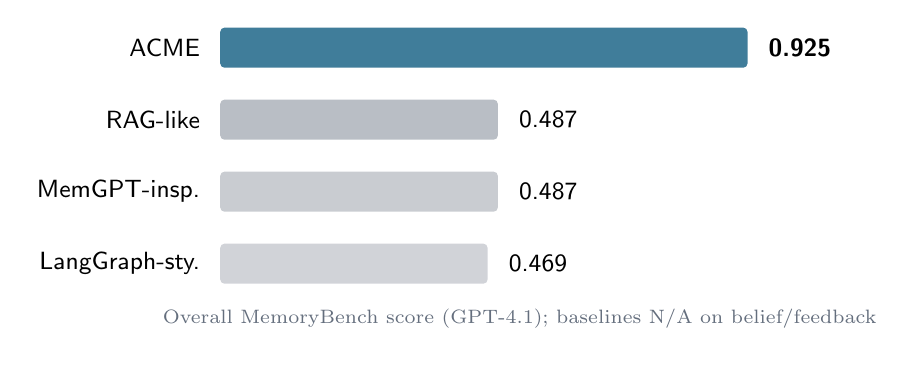
\begin{tikzpicture}[
      x=1in, y=0.36in,
      bar/.style={rounded corners=1.5pt, minimum height=0.20in, inner sep=0pt, anchor=west},
      lbl/.style={anchor=east, font=\small\sffamily},
      val/.style={anchor=west, font=\small\sffamily}
    ]
      \def\barscale{2.85}
      \node[lbl] at (0,3) {ACME};
      \node[bar, fill=acmefigblue!75, minimum width={0.925*\barscale in}] at (0.05,3) {};
      \node[val] at ($(0.05,3)+(0.925*\barscale in,0)+(0.06,0)$) {\textbf{0.925}};

      \node[lbl] at (0,2) {RAG-like};
      \node[bar, fill=acmefiggray!45, minimum width={0.487*\barscale in}] at (0.05,2) {};
      \node[val] at ($(0.05,2)+(0.487*\barscale in,0)+(0.06,0)$) {0.487};

      \node[lbl] at (0,1) {MemGPT-insp.};
      \node[bar, fill=acmefiggray!35, minimum width={0.487*\barscale in}] at (0.05,1) {};
      \node[val] at ($(0.05,1)+(0.487*\barscale in,0)+(0.06,0)$) {0.487};

      \node[lbl] at (0,0) {LangGraph-sty.};
      \node[bar, fill=acmefiggray!30, minimum width={0.469*\barscale in}] at (0.05,0) {};
      \node[val] at ($(0.05,0)+(0.469*\barscale in,0)+(0.06,0)$) {0.469};

      \node[font=\scriptsize\color{acmefiggray}, anchor=north] at (1.55,-0.5) {Overall MemoryBench score (GPT-4.1); baselines N/A on belief/feedback};
    \end{tikzpicture}
    \caption{Result summary: ACME leads primarily on feedback and belief-quality dimensions unavailable to baselines.}
    \label{fig:result-summary}
  \end{figure*}%
}


% --- Page 1: title + abstract (single column) ---
\begin{center}
  \vspace*{0.12in}
  {\sffamily\fontsize{24}{29}\selectfont\bfseries
   ACME: Adaptive Cognitive Memory Engine\par}
  \vspace{0.85em}
  {\sffamily\Large
   Externalizing Belief, Memory, and Learning from LLM Weights\par}
  \vspace{1.1em}
  {\normalsize\itshape\papertagline\par}
  \vspace{1.15em}
  {\normalsize Mohamed Kamil Bourouiba\par}
  \vspace{0.45em}
  {\small arXiv preprint draft v1.2 --- June 2026\par}
  \vspace{0.85em}
  \acmeTitleStrip
  \vspace{0.65em}
  \begin{metabox}
    \begin{minipage}{0.88\linewidth}
      \footnotesize\sffamily\color{acmefiggray}
      \textbf{Code:} \url{https://github.com/KamilBourouiba/ACME} (tag \texttt{v0.1.1-arxiv})\\
      \textbf{Project site:} \url{https://kamilbourouiba.github.io/ACME/}\\
      \textbf{Data:} \texttt{GET /api/v1/benchmark/export} (Postgres \texttt{benchmark\_runs})
    \end{minipage}
  \end{metabox}
  \vspace{0.75em}
\end{center}

\begin{abstract}
Large language models lack durable episodic memory, explicit belief
states, structured forgetting, and mechanisms to learn from failure
{[}1,2{]}. Recent systems report that agents cannot epistemically
separate observation from belief {[}50{]} and that intrinsic
\emph{epistemic agency} --- including belief updating --- remains weak
in base models {[}51{]}. We present \textbf{ACME} (Adaptive Cognitive
Memory Engine), an external cognitive substrate that treats the LLM as a
language processor while delegating persistence, confidence tracking,
contradiction handling, and self-correction to specialized engines. ACME
operationalizes: \emph{when does a collection of experiences deserve to
become a belief?} We contribute (1) a CRS-governed belief lifecycle
inspired by cognitive architecture {[}3,4{]} and truth-maintenance
systems {[}21,54{]}; (2) hybrid graph + pgvector retrieval {[}5,6{]}
with contrarian verification {[}7,8{]}; (3) \textbf{MemoryBench v3.1}
--- fourteen sandbox-isolated scenarios with RAG {[}9{]}, MemGPT
{[}10{]}, and LangGraph-style {[}11{]} baselines scored by an LLM judge
{[}12,13{]}. On Azure OpenAI GPT-4.1, ACME achieves overall
\textbf{0.925} vs \textbf{0.487} for vector-RAG (job \texttt{3b31e5e3}),
with feedback and belief-quality metrics unavailable to baselines.
Model-sensitivity runs on GPT-4.1-mini and GPT-5.4 preserve a
\textbf{+0.39--0.44} margin over RAG. Production ablations show belief
sync is essential (−0.19 overall when disabled).
\end{abstract}

\twocolumn
\raggedbottom
\emergencystretch=2em

\section{Introduction}\label{introduction}

Retrieval-augmented generation (RAG) {[}9{]} augments LLMs with document
search but does not maintain explicit epistemic states, handle
contradictory evidence, or learn from prediction failures. LongMemEval
{[}37{]} shows commercial assistants and long-context LLMs suffer
\textbf{30--60\%} accuracy drops on sustained interactive memory versus
oracle evidence --- retrieval alone is insufficient. Hindsight {[}50{]}
argues current agent memory cannot distinguish \emph{what was observed}
from \emph{what is believed}, nor maintain preference-consistent
reasoning across sessions. Reflection-Bench {[}51{]} identifies
\textbf{belief updating} and meta-reflection as core yet underdeveloped
dimensions of epistemic agency in LLMs.

Dense and hybrid retrievers {[}14,15{]} improve recall yet remain
stateless: they neither promote stable beliefs nor demote refuted
hypotheses. Agent memory frameworks --- MemGPT {[}10{]}, generative
agents {[}16{]}, Zep {[}20{]}, and LangGraph-style orchestration
{[}11{]} --- extend context windows via paging, temporal graphs, or
state graphs but lack auditable belief lifecycles and structured
feedback loops comparable to cognitive architectures {[}3,17{]}.

Episodic and semantic memory have long been distinguished in psychology
and AI {[}18,19{]}. Recent work on long-term conversational memory
(MemGPT, memory streams {[}16{]}, Zep {[}20{]}) focuses on \emph{what to
store and retrieve}, not \emph{when accumulated evidence warrants
belief}. ACME closes this gap with an explicit promotion pipeline
(Observation -\textgreater{} Inference -\textgreater{} Hypothesis
-\textgreater{} Belief) and symmetric demotion under contradiction ---
aligning with truth-maintenance and belief-revision traditions
{[}21,22{]}.

\begin{contributions}
\begin{enumerate}
\item A CRS-governed belief lifecycle with promotion and demotion under contradiction.
\item A hybrid graph + vector retrieval substrate (PostgreSQL/pgvector + Neo4j).
\item Contrarian verification for high-confidence answers.
\item MemoryBench v3.1 with scored belief and feedback metrics.
\item Production benchmark evidence across GPT-4.1, GPT-4.1-mini, and GPT-5.4.
\end{enumerate}
\end{contributions}

\textbf{Thesis.} RAG optimizes recall; ACME optimizes epistemic
state---when experiences become beliefs, how contradictions demote them,
and how outcomes close the prediction loop. Our claim is not universal
SOTA on every long-context benchmark {[}37,38{]}, but the first deployed
system with sandbox-isolated evaluation of \textbf{feedback correction}
and \textbf{belief quality (CRS)} against RAG/MemGPT/LangGraph under
reproducible production runs {[}49{]}.

\section{Related Work}\label{related-work}

\textbf{Retrieval-augmented generation.} Lewis et al.~{[}9{]}
established the retrieve-then-generate paradigm for knowledge-intensive
tasks. Subsequent systems add re-ranking {[}14{]}, query rewriting
{[}27{]}, and self-critique --- Self-RAG {[}28{]} and Corrective RAG
{[}29{]} route or revise retrieval based on generation quality. ACME
differs by persisting structured beliefs and failure traces outside the
LLM, not only refining a single-turn retrieval pass.

\textbf{Graph-augmented memory.} Knowledge-graph RAG {[}30,31{]} and
GraphRAG {[}32{]} extract communities and summaries from document
graphs. ACME maintains a \emph{live} typed graph (entities, causal
edges, tenant scope) updated on every experience, coupled with vector
recall over episodic embeddings --- hybrid retrieval akin to {[}5,6{]}
but with belief-weighted context assembly.

\textbf{Agent memory systems.} MemGPT {[}10{]} virtualizes context via
OS-inspired paging; generative agents {[}16{]} use memory streams and
reflection; LangGraph {[}11{]} composes stateful agent workflows. These
systems improve \emph{capacity} and \emph{session continuity}; ACME adds
CRS-governed belief promotion, contradiction logging, and
prediction-outcome loops absent from reference baselines in our
evaluation.

\textbf{Learning from feedback.} Reflexion {[}33{]} and ExpeL {[}34{]}
use verbal reinforcement from trial outcomes; Constitutional AI {[}35{]}
shapes behavior via principles. ACME's feedback engine ties outcome
signals to specific graph-backed beliefs, adjusting confidence and
status (e.g., Challenged -\textgreater{} Deprecated) rather than only
updating prompt-level reflections.

\textbf{Cognitive architectures.} ACT-R {[}3{]} and SOAR {[}17{]} model
declarative memory, production rules, and learning from impasse. ACME is
not a full cognitive architecture but borrows the separation of
\emph{fast reasoning} (LLM) from \emph{slow accumulative memory}
(Postgres, Neo4j, belief records) --- similar in spirit to dual-process
accounts {[}4{]} and complementary learning systems {[}36{]}.

\textbf{Evaluation of memory systems.} Benchmarks such as LongMemEval
{[}37{]}, LoCoMo {[}38{]}, MemoryBank {[}39{]}, MemoryAgentBench
{[}52{]}, and MemBench {[}53{]} stress long-horizon recall, test-time
learning, or reflective memory. Reflection-Bench {[}51{]} evaluates
belief updating as one of seven epistemic dimensions. None jointly
measure sandbox-isolated \textbf{feedback correction}, \textbf{CRS
belief quality}, and \textbf{contrarian groundedness} in a
production-deployable API. MemoryBench v3.1 fills this gap (Table 1).

\textbf{Belief-first and epistemic agent memory (concurrent work).}
TruthKeeper {[}54{]} applies dependency-aware truth maintenance to LLM
memory. MnemeBrain {[}55{]} stores beliefs with Belnap four-valued logic
and AGM-style revision. NeuSymMS {[}56{]} couples neural extraction with
symbolic TMS via rule engines. Graph-native cognitive memory
architectures {[}57{]} formalize versioned belief revision for
auditability. Hindsight {[}50{]} achieves strong LongMemEval/LoCoMo
scores via retain-recall-reflect tiers but does not expose CRS-governed
promotion thresholds or prediction-outcome loops. \textbf{ACME}
differentiates by (i) integrated seven-engine cognitive loop with
production deployment, (ii) MemoryBench v3.1 scoring belief/feedback
dimensions absent from retrieval-centric baselines, and (iii) persisted
\texttt{benchmark\_runs} for third-party reproduction.

\section{System Design}\label{system-design}

\acmeFigureLoop

\textbf{Ingestion:} LLM extraction {[}40{]} plus deterministic
normalization -\textgreater{} Neo4j entities/relations + episodic
embeddings {[}23{]}.

\textbf{Query:} Hybrid retrieval (graph neighborhood {[}24,30{]} +
pgvector cosine {[}5{]}) -\textgreater{} LLM reasoning -\textgreater{}
optional contrarian pass {[}7,8{]} when confidence \textgreater= 0.8.

\textbf{Feedback:} Outcome signals update beliefs {[}21{]}, log failures
{[}33{]}, trigger consolidation (scheduled consolidation, 6 h).

\acmeFigureBelief

\textbf{CRS (Cognitive Reliability Score)} = 40\% prediction success +
20\% temporal stability + 20\% contradiction resistance + 20\% source
diversity --- a composite reliability index analogous to calibrated
confidence under heterogeneous evidence {[}41,42{]}.

\textbf{Causal edge types:} \texttt{observed\_with}, \texttt{precedes},
\texttt{correlates}, \texttt{causes}, \texttt{disproves} ---
distinguishing correlation from causation per Pearlian and epistemic
traditions {[}43,44{]}.

\textbf{Multi-tenancy:} Postgres rows and Neo4j nodes keyed by
\texttt{tenant\_id} (header \texttt{X-Tenant-ID}).

\textbf{Ablation toggles:} \texttt{ABLATION\_DISABLE\_CONTRARIAN},
\texttt{ABLATION\_DISABLE\_BELIEF\_SYNC},
\texttt{ABLATION\_DISABLE\_VECTOR} (see Results).

\section{MemoryBench v3.1}\label{memorybench-v3.1}

Four metrics, LLM-as-judge {[}12,13{]} (semantic; keyword overlap
reported separately):

\acmeTableMetrics

\textbf{Overall} = average of all four. Baselines score 0 on
feedback/belief (N/A), capping baseline overall near 0.48--0.49.

\textbf{Fourteen scenarios:} retention, contradiction, multi-source
conflict, error injection, \textbf{knowledge update} (LongMemEval KU
{[}37{]}), long-term retention, hallucination resistance, feedback
adjustment, adversarial noise, long-horizon noise, tenant isolation,
healthcare domain transfer, multi-session recall, prediction-outcome
loop.

\textbf{Isolation:} Each scenario deletes prior benchmark-tagged
Postgres rows and Neo4j subgraph before run
(\texttt{acme/evaluation/sandbox.py}) --- preventing cross-scenario
contamination noted as a failure mode in long-horizon evals
{[}37,38,51{]}.

\textbf{Baselines:} Minimal reproducible implementations aligned with
Lewis et al.~{[}9{]} (RAG), Packer et al.~{[}10{]} (MemGPT), and
LangGraph-style state graphs {[}11{]} --- see
\texttt{docs/BASELINES.md}.

\acmeTablePositioningCapabilities

Primary reported results use the \textbf{13-scenario v3} suite (job
\texttt{3b31e5e3}, pre-\texttt{knowledge\_update}) for strict
comparability; v3.1 adds the LongMemEval-aligned knowledge-update probe.

\acmeTablePositioningInfra

\begin{keyfinding}
\textbf{Key finding.} MemoryBench v3.1 is the only evaluated suite in our comparison that jointly scores \textbf{feedback correction}, \textbf{CRS belief quality}, and \textbf{contrarian groundedness} under per-scenario sandbox isolation with a production API.
\end{keyfinding}

\section{LongMemEval (industry
benchmark)}\label{longmemeval-industry-benchmark}

To complement MemoryBench, we integrate the official
\textbf{LongMemEval} oracle split {[}37{]} (500 questions, evidence
sessions only). Chat histories are ingested via the same production
orchestrator; answers are scored with the \textbf{official LongMemEval
yes/no judge prompts} from the reference implementation.

\acmeTableLongMemEvalProtocol

\acmeTableLongMemEvalKU

\acmeTableLongMemEvalFull

\textbf{Protocol.} Each question resets sandbox state
(\texttt{longmemeval} tag). Haystack sessions are serialized as
multi-turn user/assistant transcripts and ingested as experiences. ACME
uses a \textbf{transcript-first} answer path: sessions are ranked
newest-first, the LLM reads full chat transcripts (with belief graph as
secondary context), and knowledge-update items trigger belief demotion
on superseded sources. RAG and MemGPT baselines answer from retrieved
context; an independent LLM judge (same deployment family as
MemoryBench) applies type-specific rubrics (\texttt{knowledge-update},
\texttt{temporal-reasoning}, \texttt{abstention}, etc.).

\textbf{Production runs (June 2026):} jobs \texttt{705eb2ff} (78 KU) +
\texttt{26e288da} (422 other types), API
\texttt{acme-api:longmemeval-transcript}, GPT-4.1, zero errors. Combined
summary: \texttt{benchmark-results/longmemeval-v3-combined.json}.

\textbf{Reproduction:}

\begin{Shaded}
\begin{Highlighting}[]
\FunctionTok{bash}\NormalTok{ scripts/download\_longmemeval.sh}
\FunctionTok{bash}\NormalTok{ scripts/run\_longmemeval\_prod.sh   }\CommentTok{\# Azure API}
\CommentTok{\# or locally:}
\ExtensionTok{python}\NormalTok{ scripts/run\_longmemeval.py }\AttributeTok{{-}{-}types}\NormalTok{ knowledge{-}update }\AttributeTok{{-}{-}systems}\NormalTok{ acme,rag,memgpt}
\end{Highlighting}
\end{Shaded}

Results export to \texttt{benchmark-results/longmemeval-latest.json}.
LongMemEval measures \textbf{QA accuracy over chat history}; MemoryBench
measures \textbf{belief lifecycle and feedback} --- the two benchmarks
are complementary and must not be merged into a single score.

\begin{keyfinding}
\textbf{Key finding.} On the full LongMemEval oracle split (500 Q, GPT-4.1), ACME transcript-first reaches \textbf{80.4\%} overall vs.\ 77.6\% (RAG) and 78.0\% (MemGPT), with the largest gains on \texttt{knowledge-update} (89.7\% vs.\ 85.9\%) and \texttt{temporal-reasoning} (68.4\% vs.\ 60.2\%) while preserving MemoryBench belief/feedback advantages (Section 6).
\end{keyfinding}

\section{Experimental Setup}\label{experimental-setup}

\acmeTableSetup

\textbf{Model-sensitivity runs} additionally use GPT-4.1-mini and
GPT-5.4 (same endpoint family; GPT-5.4 requires
\texttt{max\_completion\_tokens} API parameter).

\FloatBarrier

\section{Results}\label{results}

\textbf{Run metadata:} API revision \texttt{acme-api-\/-membenchfix};
compare job\\
\texttt{3b31e5e3-72b1-4ce3-b6c2-848cf94e4128}; duration 725 s; zero
scenario failures.

\acmeResultSummary

\acmeTableMain

\emph{Baselines exclude feedback/belief in overall (not applicable).
Scores rounded to three decimals from persisted \texttt{benchmark\_runs}
export.}

\begin{keyfinding}
\textbf{Key finding.} ACME's advantage comes primarily from \textbf{feedback correction} and \textbf{belief quality}, rather than from raw retention alone. ACME gains \textbf{+0.44} overall vs RAG on GPT-4.1 while retention and groundedness remain competitive ($\geq 0.90$) across systems [9,32].
\end{keyfinding}

\subsection{Model sensitivity
(GPT-4.1-mini)}\label{model-sensitivity-gpt-4.1-mini}

Job \texttt{107d02c0}, 639 s. ACME retains \textbf{+0.39} overall vs RAG
(0.858 vs 0.473). Feedback stays at 1.000 and belief at 0.700 ---
cognitive layers compensate when the base model is weaker {[}4,36{]}.

\acmeTableMini

\subsection{Model sensitivity
(GPT-5.4)}\label{model-sensitivity-gpt-5.4}

Job \texttt{eb68f028}, 620 s. ACME \textbf{0.873} vs RAG \textbf{0.474}
(\textbf{+0.40}).

\acmeTableGptFiveFour

Belief quality remains \textbf{\textasciitilde0.70} across all three LLM
tiers --- suggesting the external belief substrate {[}3,21{]} is
comparatively stable while retention/groundedness track model capability
{[}12{]}.

\subsection{Component ablations}\label{component-ablations}

We disable one cognitive layer at a time via environment flags
(\texttt{scripts/run\_ablation\_prod.sh}). Table 2 reports ACME-only
MemoryBench v3.1 scores (no baseline compare --- 4x cost reduction per
ablation).

\acmeTableAblations

\emph{Full ACME row from 13-scenario compare (job \texttt{3b31e5e3}).
Ablation rows from ACME-only runs on GPT-4.1 (24 June 2026, premium
ingress, stamp \texttt{20260624213154}).}

\begin{keyfinding}
\textbf{Key finding.} Disabling belief sync collapses belief quality to \textbf{0.000} and overall score by \textbf{$-$0.19}, confirming the belief engine as the primary differentiator. Contrarian and vector ablations each reduce overall by only \textbf{$-$0.002}.
\end{keyfinding}

\section{Limitations}\label{limitations}

\begin{keyfinding}
\textbf{Key limitations.}
\begin{itemize}
\item LLM judge and extractor introduce variance [12,13]; we report sandbox-isolated runs with persisted \texttt{benchmark\_runs}.
\item Scenarios emphasize SaaS churn/latency plus one healthcare transfer set; broader domains and multilingual evals needed [37,38].
\item Baselines are reference implementations, not full upstream MemGPT/LangGraph codebases [10,11].
\item Production API requires API key for benchmark endpoints.
\item CRS weights are hand-tuned; calibration against human epistemic judgments [41] is future work.
\item \textbf{LongMemEval routing.} Transcript-first answering (newest session wins) is enabled for the LongMemEval adapter to resolve knowledge-update items; it is not the default MemoryBench query path (graph + CRS). This is intentional benchmark alignment [37] but blurs the single-pipeline story --- hybrid routing by question type is future work.
\item \textbf{Multi-session gap.} On LongMemEval oracle (500 Q), RAG slightly exceeds ACME on \texttt{multi-session} (78.9\% vs.\ 74.4\%), suggesting dense vector recall still wins when evidence is spread across many sessions without explicit temporal conflict.
\item \textbf{Abstention.} ACME abstention accuracy on LongMemEval probe questions remains $\sim$50\% (KU subset); conflating unrelated entities (e.g.\ Dr.\ Smith vs.\ Dr.\ Johnson) needs dedicated abstention prompts and entity-scope checks.
\end{itemize}
\end{keyfinding}

\section{Conclusion}\label{conclusion}

ACME shows that externalizing belief and learning from LLM weights
yields stronger cognitive memory than vector RAG or lightweight
agent-memory baselines on MemoryBench, especially for feedback-driven
correction and auditable belief quality. On the official LongMemEval
oracle split (500 Q, GPT-4.1), transcript-first ACME reaches
\textbf{80.4\%} overall vs.~\textbf{77.6\%} (RAG), with the largest
margins on knowledge-update and temporal-reasoning types. The consistent
\textbf{+0.39--0.44} margin over RAG on MemoryBench across GPT-4.1,
GPT-4.1-mini, and GPT-5.4 supports the hypothesis that explicit belief
lifecycle management {[}21,22,54,55{]} complements --- rather than
replaces --- advances in base model capability {[}1,47{]}. Concurrent
belief-memory systems {[}50,54,56,57{]} validate the problem direction;
ACME contributes reproducible production evidence that epistemic layers
--- not retrieval alone --- drive the measured gap on MemoryBench, while
benchmark-specific transcript routing closes industry QA gaps without
abandoning the cognitive substrate.

\acmeBackMatterBegin
\acmeReferencesBegin

\section{References}\label{references}

\begin{enumerate}
\def\labelenumi{\arabic{enumi}.}
\tightlist
\item
  Bommasani, R. et al.~On the Opportunities and Risks of Foundation
  Models. \emph{arXiv:2108.07258}, 2021.
\item
  McKenna, B. et al.~Towards Reliable Generation: Rethinking
  Faithfulness and Hallucination in LLMs. \emph{Findings of ACL}, 2024.
\item
  Anderson, J. R., Bothell, D., Byrne, M. D., Douglass, S., Lebiere, C.,
  \& Qin, Y. An Integrated Theory of the Mind. \emph{Psychological
  Review}, 111(4), 1036--1060, 2004.
\item
  Evans, J. S. B. T. \& Stanovich, K. E. Dual-Process Theories of Higher
  Cognition. \emph{Perspectives on Psychological Science}, 8(3),
  223--241, 2013.
\item
  Gao, L. et al.~Retrieval-Augmented Generation for Large Language
  Models: A Survey. \emph{arXiv:2312.10997}, 2023.
\item
  Wang, X. et al.~Searching for Best Practices in Retrieval-Augmented
  Generation. \emph{arXiv:2407.01219}, 2024.
\item
  Madaan, A. et al.~Self-Refine: Iterative Refinement with
  Self-Feedback. \emph{NeurIPS}, 2023.
\item
  Saunders, W. et al.~Self-Critiquing Models for Assisting Human
  Evaluators. \emph{arXiv:2206.05802}, 2022.
\item
  Lewis, P. et al.~Retrieval-Augmented Generation for
  Knowledge-Intensive NLP Tasks. \emph{NeurIPS}, 2020.
\item
  Packer, C. et al.~MemGPT: Towards LLMs as Operating Systems.
  \emph{arXiv:2310.08560}, 2023.
\item
  LangChain. LangGraph: Building Stateful, Multi-Actor Applications with
  LLMs. Documentation, 2024. https://langchain-ai.github.io/langgraph/
\item
  Zheng, L. et al.~Judging LLM-as-a-Judge with MT-Bench and Chatbot
  Arena. \emph{NeurIPS}, 2023.
\item
  Liu, Y. et al.~G-Eval: NLG Evaluation using GPT-4 with Better Human
  Alignment. \emph{EMNLP}, 2023.
\item
  Karpukhin, V. et al.~Dense Passage Retrieval for Open-Domain Question
  Answering. \emph{EMNLP}, 2020.
\item
  Khattab, O. \& Zaharia, M. ColBERT: Efficient and Effective Passage
  Search via Contextualized Late Interaction. \emph{SIGIR}, 2020.
\item
  Park, J. S. et al.~Generative Agents: Interactive Simulacra of Human
  Behavior. \emph{UIST}, 2023.
\item
  Laird, J. E. The SOAR Cognitive Architecture. \emph{MIT Press}, 2012.
\item
  Tulving, E. Episodic and Semantic Memory. In \emph{Organization of
  Memory}, 1972.
\item
  Schacter, D. L. \& Tulving, E. Memory Systems. \emph{MIT Press}, 1994.
\item
  Rasmussen, D. et al.~Zep: A Temporal Knowledge Graph Architecture for
  Agent Memory. \emph{arXiv:2501.13956}, 2025.
\item
  Doyle, J. A Truth Maintenance System. \emph{Artificial Intelligence},
  12(3), 231--272, 1979.
\item
  Gardenfors, P. \emph{Knowledge in Flux: Modeling the Dynamics of
  Epistemic States}. MIT Press, 1988.
\item
  pgvector. Open-source vector similarity search for PostgreSQL.
  https://github.com/pgvector/pgvector
\item
  Neo4j, Inc.~Neo4j Graph Database. https://neo4j.com/
\item
  Parisi, G. I. et al.~Continual Lifelong Learning with Neural Networks:
  A Review. \emph{Neural Networks}, 113, 54--71, 2019.
\item
  Kemper, N. \& Jankowski, S. Forgetting in Deep Learning --- A Survey.
  \emph{arXiv:2307.09218}, 2023.
\item
  Ma, X. et al.~Query Rewriting for Retrieval-Augmented Large Language
  Models. \emph{EMNLP}, 2023.
\item
  Asai, A. et al.~Self-RAG: Learning to Retrieve, Generate, and Critique
  through Self-Reflection. \emph{ICLR}, 2024.
\item
  Yan, S. et al.~Corrective Retrieval Augmented Generation.
  \emph{arXiv:2401.15884}, 2024.
\item
  Edge, D. et al.~From Local to Global: A Graph RAG Approach to
  Query-Focused Summarization. \emph{arXiv:2404.16130}, 2024 (Microsoft
  GraphRAG).
\item
  Wang, M. et al.~Knowledge Graph Prompting for Multi-Document Question
  Answering. \emph{EMNLP}, 2023.
\item
  Edge, D. et al.~GraphRAG: Unlocking LLM Discovery on Narrative Private
  Data. Microsoft Research, 2024.
\item
  Shinn, N. et al.~Reflexion: Language Agents with Verbal Reinforcement
  Learning. \emph{NeurIPS}, 2023.
\item
  Zhao, A. et al.~ExpeL: LLM Agents Are Experiential Learners.
  \emph{AAAI}, 2024.
\item
  Bai, Y. et al.~Constitutional AI: Harmlessness from AI Feedback.
  \emph{arXiv:2212.08073}, 2022.
\item
  McClelland, J. L., McNaughton, B. L., \& O'Reilly, R. C. Why There Are
  Complementary Learning Systems in the Hippocampus and Neocortex.
  \emph{Psychological Review}, 102(3), 419--457, 1995.
\item
  Wu, Y. et al.~LongMemEval: Benchmarking Long-Term Memory in LLMs.
  \emph{arXiv:2410.10813}, 2024.
\item
  Maharana, D. et al.~Evaluating Very Long-Term Conversational Memory of
  LLM Agents (LoCoMo). \emph{ACL}, 2024.
\item
  Zhong, W. et al.~MemoryBank: Enhancing Large Language Models with
  Long-Term Memory. \emph{AAAI}, 2024.
\item
  Wang, X. et al.~Text2KG: A Survey on Knowledge Graph Construction from
  Text. \emph{arXiv:2404.09425}, 2024.
\item
  Guo, C. et al.~On Calibration of Modern Neural Networks. \emph{ICML},
  2017.
\item
  Kadavath, S. et al.~Language Models (Mostly) Know What They Know.
  \emph{arXiv:2207.05221}, 2022.
\item
  Pearl, J. \emph{Causality: Models, Reasoning, and Inference}.
  Cambridge University Press, 2009.
\item
  Halpern, J. Y. \emph{Actual Causality}. MIT Press, 2016.
\item
  Ji, Z. et al.~Survey of Hallucination in Natural Language Generation.
  \emph{ACM Computing Surveys}, 55(12), 2023.
\item
  Min, S. et al.~FactScore: Fine-grained Atomic Evaluation of Factual
  Precision in Long Form Text Generation. \emph{EMNLP}, 2023.
\item
  OpenAI. GPT-4.1 Model Card and System Documentation, 2025.
\item
  Neelakantan, A. et al.~Text and Code Embeddings by Contrastive
  Pre-Training. \emph{arXiv:2201.10005}, 2022.
\item
  Kamil Bourouiba. ACME: Adaptive Cognitive Memory Engine (code and
  benchmarks). https://github.com/KamilBourouiba/ACME, 2026.
\item
  Latif, E. et al.~Hindsight is 20/20: Building Agent Memory that
  Retains, Recalls, and Reflects. \emph{arXiv:2512.12818}, 2025.
\item
  Chen, Y. et al.~Reflection-Bench: Evaluating Epistemic Agency in Large
  Language Models. \emph{arXiv:2410.16270}, 2024.
\item
  MemoryAgentBench authors. Evaluating Memory in LLM Agents via
  Incremental Multi-Turn Interactions. \emph{arXiv:2507.05257}, 2025.
\item
  Ai, J. et al.~MemBench: Towards More Comprehensive Evaluation on the
  Memory of LLM-based Agents. \emph{arXiv:2506.21605}, 2025.
\item
  TruthKeeper authors. TruthKeeper: A Curated Memory Architecture for
  LLMs with Dependency-Aware Truth Maintenance. \emph{arXiv preprint},
  2024.
\item
  MnemeBrain. Belief-State Memory for AI Agents.
  https://github.com/mnemebrain/mnemebrain-lite, 2025.
\item
  NeuSymMS authors. NeuSymMS: A Hybrid Neuro-Symbolic Memory System for
  LLM Agents. \emph{arXiv:2605.17596}, 2026.
\item
  Graph-Native Cognitive Memory authors. Formal Belief Revision
  Semantics for Versioned Memory Architectures. \emph{arXiv:2603.17244},
  2026.
\item
  Alchourron, C. E., Gardenfors, P., \& Makinson, D. On the Logic of
  Theory Change: Partial Meet Contraction and Revision Functions.
  \emph{Journal of Symbolic Logic}, 50(2), 510--530, 1985.
\end{enumerate}

\acmeReferencesEnd

\begingroup\footnotesize

\section{Appendix A: Reproduction}
\label{appendix-a-reproduction}

\begin{tcolorbox}[
  enhanced,
  colback=bannerbg,
  colframe=keyborder!25,
  boxrule=0.35pt,
  arc=3pt,
  left=8pt, right=8pt, top=6pt, bottom=6pt
]
\begin{Verbatim}[fontsize=\scriptsize]
git clone https://github.com/KamilBourouiba/ACME.git && cd ACME
pip install -e ".[dev]"
pytest tests/test_benchmark_gate.py tests/test_memorybench.py -q
# Production (requires API key):
./azure/configure-premium-ingress.sh
./scripts/run_prod_benchmark.sh
./scripts/run_model_benchmark.sh gpt-4.1-mini   # optional model sweep
./scripts/run_ablation_prod.sh                # component ablations
\end{Verbatim}
\end{tcolorbox}

\section{Appendix B: Data Availability}
\label{appendix-b-data-availability}

Benchmark payloads are stored in PostgreSQL table
\texttt{benchmark\_runs} (columns: \texttt{overall\_score},
\texttt{retention\_score}, \texttt{belief\_quality\_score},
\texttt{payload JSONB}, \texttt{created\_at}). Export via
\texttt{GET /api/v1/benchmark/export}. Full run tables are documented in
\texttt{docs/BENCHMARK\_RESULTS.md}\textasciitilde{[}49{]}.

\endgroup

\end{document}
